% Symbolic Pipeline: Data Flow, Wolfram Modules, JSON Specification, and Python Classes
% Source: docs/source/pipeline.md (migrated to LaTeX)
% Uses macros from preamble.tex

\section{Symbolic Pipeline}
\label{sec:pipeline}

TIDAL implements a two-stage pipeline that transforms symbolic Lagrangians into numerical PDE simulations.
\textbf{No physics is hardcoded} --- all equation structure comes from symbolic derivation.

\subsection{Data Flow}

\begin{center}
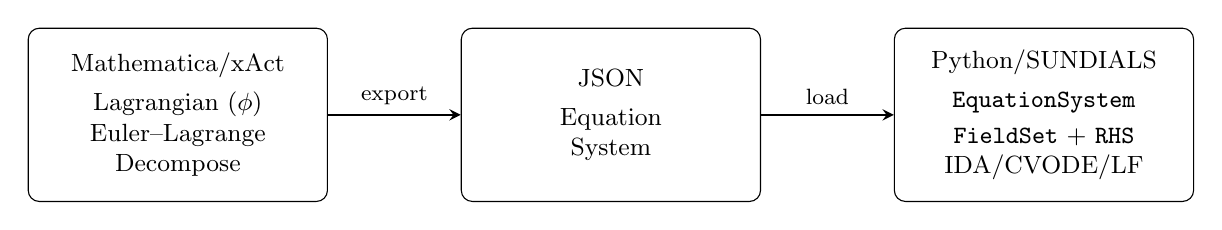
\begin{tikzpicture}[
  box/.style={draw, rounded corners, minimum width=3.8cm, minimum height=2.2cm, align=center, font=\small},
  arr/.style={->, thick, >=stealth},
]
\node[box] (wolf) at (0,0)     {Mathematica/xAct\\[3pt]Lagrangian $\lag(\phi)$\\Euler--Lagrange\\Decompose};
\node[box] (json) at (5.5,0)   {JSON\\[3pt]Equation\\System};
\node[box] (py)   at (11,0)    {Python/SUNDIALS\\[3pt]\texttt{EquationSystem}\\[2pt]\texttt{FieldSet} + \texttt{RHS}\\IDA/CVODE/LF};
\draw[arr] (wolf) -- node[above, font=\footnotesize] {export} (json);
\draw[arr] (json) -- node[above, font=\footnotesize] {load} (py);
\end{tikzpicture}
\end{center}

\textbf{Stage~1 (Mathematica/xAct)} derives field equations symbolically from a Lagrangian.
\textbf{Stage~2 (Python/SUNDIALS + numpy)} loads the specification and runs a numerical simulation.

\subsection{Wolfram Modules}

\begin{table}[htbp]
\centering
\begin{tabular}{@{}lp{4cm}p{5.5cm}@{}}
\toprule
Module & Purpose & Key Function \\
\midrule
\texttt{CommonUtilities.wl}    & Shared helpers: CD-to-Derivative conversion, Christoffel/epsilon evaluation & \texttt{ConvertCDToDerivatives}, \texttt{EvaluateChristoffelComponents} \\
\texttt{EulerLagrange.wl}      & Derive equations of motion from a Lagrangian & \texttt{EulerLagrangeEquation[L, field, cd]} \\
\texttt{ComponentDecompose.wl}  & Convert tensor EOM to scalar component equations & \texttt{DecomposeToComponents[eom, field, chart, additionalFields]} \\
\texttt{ExportJSON.wl}          & Serialize component equations to JSON & \texttt{BuildMultiFieldJSONStructure[fieldEquations, metadata]} \\
\texttt{Linearize.wl}           & Perturbation theory (xPert) for linearized gravity & \texttt{LinearizeTensorExpression[expr]} \\
\bottomrule
\end{tabular}
\end{table}

\subsection{Canonicalization of Deferred Derived Fields}
\label{subsec:canonicalization}

Multi-field theories that use \emph{derived tensors} such as the Maxwell
field strength $F_{\mu\nu} = \partial_\mu A_\nu - \partial_\nu A_\mu$ or
the torsion field strength $F^{\text{tor}}_{\mu\nu\rho} = \partial T$
require special handling in the linearization pipeline. TIDAL's approach
is to keep these abstract through \texttt{xPert} (issue \#218) and only
expand them once the perturbation expansion is complete. This
\emph{deferred-field} pattern avoids a cancellation pathology that
otherwise corrupts photon equations of motion when $F$ is expanded before
\texttt{xPert} (a50b11f).

The deferred fields must then be canonicalized before component
decomposition. From v0.29.3 to v0.29.4 this step was guarded by three
increasingly layered workarounds, all collapsed into a single uniform
path in v0.30.0 (commit \texttt{4fef016}). The history is documented
here because future maintainers working on the canonical pipeline need
to understand why it looks the way it does.

\paragraph{Historical pathology.} The pre-v0.30.0 pipeline applied
\texttt{ContractMetric[ToCanonical[Total[batch]], metric]} per batch of
$\sim 20$ terms from $L^{(2)}$, accumulating the results. This is
semantically unsafe for any expression where tensor contractions span
multiple \texttt{Plus}-terms:

\begin{itemize}
  \item \textbf{\#218 — photon EOM merge.} With $F$ still abstract,
    \texttt{ToCanonical} merged antisymmetric Maxwell contractions across
    batches and collapsed the four-component photon into a constraint.
    Fixed in \texttt{a50b11f} by deferring $F$ upstream of \texttt{xPert}.
  \item \textbf{\#250 — h\textunderscore 5 fragment.} The graviton
    kinetic contraction $\partial h_{ij} \partial h^{ij}$ spans many
    \texttt{Plus}-terms. Batched \texttt{ToCanonical} saw only trace-like
    fragments in each batch and collapsed $h_5 = h_{xy}$
    off-diagonal polarization into the constraint set. Fixed in
    \texttt{9f496ef} by building a parallel \texttt{LagrangianFullExpand}
    copy with $F$ pre-expanded and canonicalized in a single pass.
  \item \textbf{\#255 — torsion cross-sector interference.} When abstract
    $F^{\text{tor}}$ and $F$ both appeared, \texttt{ToCanonical}'s global
    tensor symmetries halved non-trace $h_{ab}$ coefficients. Fixed in
    \texttt{51a36fd} by bypassing \texttt{ToCanonical} entirely for
    torsion-deferred theories.
\end{itemize}

\paragraph{Root cause.} All three symptoms share a single root: running
\texttt{ToCanonical} on $L^{(2)}$ while abstract deferred tensors are
still present. Per-term batching is structurally unsafe for any
cross-term kinetic structure. The batching existed only as a performance
optimization against the super-linear cost of \texttt{ToCanonical}; it
traded correctness for throughput.

\paragraph{v0.30.0 unified pipeline.} The fix has two steps:

\begin{enumerate}
  \item \textbf{Expand deferred fields before canonicalization.}
    \texttt{\_wls\_deferred\_field\_expand} runs first, substituting
    $F \to d(a)$, $F^{\text{tor}} \to d(t)$. All tensors are then
    concrete derivative products with no abstract antisymmetric
    structure.
  \item \textbf{Single-pass canonicalization with cost-based fallback.}
\begin{verbatim}
Module[{nTerms, tStart, canonical},
  nTerms = If[Head[l2Raw] === Plus, Length[l2Raw], 1];
  tStart = AbsoluteTime[];
  canonical = TimeConstrained[
    ContractMetric[ToCanonical[l2Raw], metric],
    15.0,
    $Aborted
  ];
  If[canonical === $Aborted,
    (* #201-class theories: fall back to Expand-only.  Downstream
       DecomposeScalarExpression canonicalizes per-component. *)
    l2Raw = Expand[l2Raw],
    l2Raw = canonical;
  ];
];
\end{verbatim}
\end{enumerate}

\paragraph{Why the Expand-only fallback is safe.} The downstream
\texttt{ComponentDecompose} step runs \texttt{ToBasis} and
\texttt{TraceBasisDummy} at per-component scalar level. Scalar
expressions are much smaller than the full $L^{(2)}$ and
\texttt{ToCanonical} there is cheap. The non-canonical \texttt{Expand}
output is then canonicalized per-component before Hamiltonian extraction,
preserving correctness. Issue \#201 (non-minimal $\tilde R_{\mu\nu} F^{\mu\nu}$
coupling, 5000+ terms, 467s under the old code) uses this fallback in
production and produces a correct Hamiltonian.

\paragraph{Scope of the fix.} All three workarounds
(\texttt{LagrangianFullExpand}, \texttt{has\_torsion\_deferred} bypass,
\texttt{lagForCanon} conditional) and the batching loop itself were
deleted in v0.30.0 — $\sim 175$ lines of code removed. The
\texttt{a50b11f} F-deferral upstream of \texttt{xPert} remains in place
as an orthogonal xPert-layer concern. Verification: all four tracked
deferred-field JSONs (\texttt{gertsenshtein}, \texttt{torsion\_dark\_photon},
\texttt{graviton\_torsion}, \texttt{torsion\_gertsenshtein\_propagating})
re-derive with bitwise-identical coefficients to v0.29.4 — only
\texttt{derivation\_hash} changes. See \texttt{CHANGELOG.md} entry
\textbf{0.30.0} for the full trail.

\subsection{JSON Specification}

The JSON file is the contract between symbolic and numerical layers:

\begin{lstlisting}[style=json]
{
  "spacetime": { "dimension": 2, "signature": [-1, 1],
                 "coordinates": ["t", "x"] },
  "fields": [
    { "name": "phi_0", "index": 0, "is_dynamical": true }
  ],
  "equations": [
    {
      "field": "phi_0",
      "lhs": { "expression": "d2_t(phi_0)", "order": { "time": 2 } },
      "rhs": {
        "type": "linear_combination",
        "terms": [
          { "coefficient": 1.0, "operator": "laplacian",
            "field": "phi_0" },
          { "coefficient": -1.0,
            "coefficient_symbolic": "-m2",
            "operator": "identity", "field": "phi_0" }
        ]
      }
    }
  ],
  "metadata": { "lagrangian_expr": "1/2 (d phi)^2 - 1/2 m^2 phi^2" }
}
\end{lstlisting}

For the full schema reference, see the JSON Schema Guide.\footnote{\url{https://github.com/WilliamRoyce/tidal/blob/main/docs/JSON\_SCHEMA\_GUIDE.md}}

\subsection{Python-Side Classes}

\subsubsection{\texttt{EquationSystem} (\texttt{json\_loader.py})}

Parsed equation specification loaded from JSON:

\begin{lstlisting}[style=python]
from tidal.symbolic.json_loader import load_equation_system

# Load equation specification
spec = load_equation_system("examples/data/klein_gordon_1d.json")

# Runtime parameter overrides are passed to the solver
# via --param or programmatically
\end{lstlisting}

Key features:
\begin{itemize}
  \item Frozen dataclass for immutability
  \item Auto-computes mass/coupling matrices from equation terms
  \item Preserves symbolic coefficient expressions for runtime parameter sweeps
\end{itemize}

\subsubsection{Solver Classes (\texttt{tidal/solver/})}

The solver layer builds the numerical system from the equation specification:

\begin{itemize}
  \item \texttt{FieldSet.from\_spec(spec)} --- field storage and boundary conditions
  \item \texttt{CoefficientEvaluator(spec)} --- 4-level cached coefficient resolution
  \item \texttt{RHSEvaluator(spec)} --- evaluates RHS from JSON terms (no hardcoded physics)
  \item \texttt{StateLayout.from\_spec(spec)} --- maps fields to state vector slots
\end{itemize}

Supports second-order (wave), first-order, and constraint (order-0) equations in the same system.

\subsection{Supported Operators}

Operators map JSON terms to numpy spatial operations (finite-difference stencils). All support cross-field references.

\begin{table}[htbp]
\centering
\begin{tabular}{@{}lll@{}}
\toprule
Operator & Min Dim & Description \\
\midrule
\texttt{identity}                     & 1D     & Field value (mass/coupling terms) \\
\texttt{laplacian}                    & 1D     & Full spatial Laplacian \\
\texttt{laplacian\_x}, \texttt{\_y}, \texttt{\_z} & 1D/2D/3D & Directional second derivative \\
\texttt{gradient\_x}, \texttt{\_y}, \texttt{\_z}  & 1D/2D/3D & Directional first derivative \\
\texttt{cross\_derivative\_xy}, \texttt{\_xz}, \texttt{\_yz} & 2D/3D & Mixed partial derivative \\
\texttt{first\_derivative\_t}         & 1D     & Time derivative (friction/damping terms) \\
\texttt{biharmonic}                   & 1D     & Fourth-order Laplacian \\
\bottomrule
\end{tabular}
\end{table}

\subsection{Christoffel Auto-Detection}

For curvilinear coordinates, the pipeline automatically detects whether Christoffel symbols are needed:

\begin{itemize}
  \item \textbf{Constant metric} (flat Minkowski, static conformal): all Christoffels $= 0$
  \item \textbf{Non-constant metric} (polar, spherical, expanding universe): computed from standard formula
\end{itemize}

This is controlled by \texttt{DecomposeToComponents} with the \texttt{"MetricMatrix"} option. Override with \texttt{"ComputeChristoffels"~->~True/False} for explicit control.

\subsection{Mass/Coupling Matrix Auto-Computation}

As of Phase~12, mass and coupling matrices are \textbf{automatically computed} from equation terms on both the Wolfram and Python sides:

\begin{itemize}
  \item \textbf{Convention}: $\texttt{matrix}[i][j] = -(\text{coefficient of identity}(\text{field}\_j) \text{ in equation}\_i)$
  \item \textbf{Symbolic preservation}: \texttt{mass\_matrix\_symbolic} / \texttt{coupling\_matrix\_symbolic} preserve exact Mathematica expressions
  \item \textbf{Runtime sweeps}: Override symbolic coefficients via \texttt{parameters=\{"m2":~1.0,~"g":~0.5\}} without regenerating JSON
\end{itemize}
